% questions.tex —— 2023 年·全国甲卷·文科 · 题目内容片段（无答案）
% 由 tools/generate_projects.py 依来源总账自 2023/2023_数学真题_全国甲文_试题.md 生成，勿手改（改源 MD 后重跑）


\par\medskip

\gkpart{一、单选题}

\begin{question}
\gkti{1}设全集 $U=\{1,2,3,4,5\}$，集合 $M=\{1,4\}$，$N=\{2,5\}$，则 $N\cup\complement_U M=$\mbox{（　　）}

\begin{gkopts}(4)
\task A．$\{2,3,5\}$
\task B．$\{1,3,4\}$
\task C．$\{1,2,4,5\}$
\task D．$\{2,3,4,5\}$
\end{gkopts}

\end{question}
\begin{question}
\gkti{2}$\dfrac{5(1+\mathrm i^3)}{(2+\mathrm i)(2-\mathrm i)}=$\mbox{（　　）}

\begin{gkopts}(4)
\task A．$-1$
\task B．$1$
\task C．$1-\mathrm i$
\task D．$1+\mathrm i$
\end{gkopts}

\end{question}
\begin{question}
\gkti{3}已知向量 $\boldsymbol a=(3,1)$，$\boldsymbol b=(2,2)$，则 $\cos\langle\boldsymbol a+\boldsymbol b,\boldsymbol a-\boldsymbol b\rangle=$\mbox{（　　）}

\begin{gkopts}(2)
\task A．$\dfrac1{17}$
\task B．$\dfrac{\sqrt{17}}{17}$
\task C．$\dfrac{\sqrt5}{5}$
\task D．$\dfrac{2\sqrt5}{5}$
\end{gkopts}

\end{question}
\begin{question}
\gkti{4}某校文艺部有 $4$ 名学生，其中高一、高二年级各 $2$ 名．从这 $4$ 名学生中随机选 $2$ 名组织校文艺汇演，则这 $2$ 名学生来自不同年级的概率为\mbox{（　　）}

\begin{gkopts}(4)
\task A．$\dfrac16$
\task B．$\dfrac13$
\task C．$\dfrac12$
\task D．$\dfrac23$
\end{gkopts}

\end{question}
\begin{question}
\gkti{5}记 $S_n$ 为等差数列 $\{a_n\}$ 的前 $n$ 项和．若 $a_2+a_6=10$，$a_4a_8=45$，则 $S_5=$\mbox{（　　）}

\begin{gkopts}(4)
\task A．$25$
\task B．$22$
\task C．$20$
\task D．$15$
\end{gkopts}

\Needspace{0.4\textheight}
\end{question}
\begin{question}
\gkti{6}执行如图的程序框图，则输出的 $B=$\mbox{（　　）}
\nopagebreak[4]
\begin{center}% 2023 全国甲卷文科 6：程序框图
% 源图流程：输入 n=3,A=1,B=2,k=1；当 k<=n 时依次更新 A、B、k 并折返判断；
% 条件不成立时输出 B。源图所有边均为实线。
\begin{tikzpicture}[font=\footnotesize, >=Stealth, node distance=2.2mm, line width=0.4pt,
  box/.style={draw, minimum height=1.5em, minimum width=5.8em, inner xsep=6pt},
  term/.style={draw, rounded corners=6pt, minimum height=1.5em, inner xsep=8pt},
  io/.style={draw, trapezium, trapezium left angle=70, trapezium right angle=110,
             minimum height=1.5em, inner xsep=3pt},
  dec/.style={draw, diamond, aspect=2.6, inner sep=1.5pt}]
  \node[term] (start) {开始};
  \node[io, below=of start] (input) {输入 $n=3,A=1,B=2,k=1$};
  \coordinate[below=1mm of input] (merge);
  \node[dec, below=1mm of merge] (cond) {$k\leqslant n$};
  \node[box, below=of cond] (stepa) {$A=A+B$};
  \node[box, below=of stepa] (stepb) {$B=A+B$};
  \node[box, below=of stepb] (stepk) {$k=k+1$};
  \node[io, below=2.5mm of stepk] (output) {输出 $B$};
  \node[term, below=of output] (end) {结束};

  % 主流程与“是”分支
  \draw[->] (start) -- (input);
  \draw[->] (input) -- (cond);
  \draw[->] (cond) -- node[right, pos=0.38] {是} (stepa);
  \draw[->] (stepa) -- (stepb);
  \draw[->] (stepb) -- (stepk);

  % k=k+1 后从左侧折返，在输入框与判断框之间重新汇入
  \draw[->] (stepk.west) -- ++(-14mm,0) |- (merge);

  % “否”从菱形右侧绕至输出框上方，再向下进入输出框
  \coordinate[right=16mm of cond] (no-right);
  \coordinate[above=4mm of output] (out-merge);
  \draw (cond.east) -- node[above, pos=0.38] {否} (no-right) |- (out-merge);
  \draw[->] (out-merge) -- (output.north);
  \draw[->] (output) -- (end);
\end{tikzpicture}
\end{center}
\nopagebreak[4]
\begin{gkopts}(4)
\task A．$21$
\task B．$34$
\task C．$55$
\task D．$89$
\end{gkopts}

\end{question}
\begin{question}
\gkti{7}设 $F_1$，$F_2$ 为椭圆 $C:\dfrac{x^2}{5}+y^2=1$ 的两个焦点，点 $P$ 在 $C$ 上，若 $\overrightarrow{PF_1}\cdot\overrightarrow{PF_2}=0$，则 $|PF_1|\cdot|PF_2|=$\mbox{（　　）}

\begin{gkopts}(4)
\task A．$1$
\task B．$2$
\task C．$4$
\task D．$5$
\end{gkopts}

\end{question}
\begin{question}
\gkti{8}曲线 $y=\dfrac{\mathrm e^x}{x+1}$ 在点 $\left(1,\dfrac{\mathrm e}{2}\right)$ 处的切线方程为\mbox{（　　）}

\begin{gkopts}(1)
\task A．$y=\dfrac{\mathrm e}{4}x$
\task B．$y=\dfrac{\mathrm e}{2}x$
\task C．$y=\dfrac{\mathrm e}{4}x+\dfrac{\mathrm e}{4}$
\task D．$y=\dfrac{\mathrm e}{2}x+\dfrac{3\mathrm e}{4}$
\end{gkopts}

\end{question}
\begin{question}
\gkti{9}已知双曲线 $C:\dfrac{x^2}{a^2}-\dfrac{y^2}{b^2}=1$（$a>0$，$b>0$）的离心率为 $\sqrt5$，$C$ 的一条渐近线与圆 $(x-2)^2+(y-3)^2=1$ 交于 $A$，$B$ 两点，则 $|AB|=$\mbox{（　　）}

\begin{gkopts}(2)
\task A．$\dfrac{\sqrt5}{5}$
\task B．$\dfrac{2\sqrt5}{5}$
\task C．$\dfrac{3\sqrt5}{5}$
\task D．$\dfrac{4\sqrt5}{5}$
\end{gkopts}

\end{question}
\begin{question}
\gkti{10}在三棱锥 $P-ABC$ 中，$\triangle ABC$ 是边长为 $2$ 的等边三角形，$PA=PB=2$，$PC=\sqrt6$，则该棱锥的体积为\mbox{（　　）}

\begin{gkopts}(4)
\task A．$1$
\task B．$\sqrt3$
\task C．$2$
\task D．$3$
\end{gkopts}

\end{question}
\begin{question}
\gkti{11}已知函数 $f(x)=\mathrm e^{-(x-1)^2}$．记 $a=f\left(\dfrac{\sqrt2}{2}\right)$，$b=f\left(\dfrac{\sqrt3}{2}\right)$，$c=f\left(\dfrac{\sqrt6}{2}\right)$，则\mbox{（　　）}

\begin{gkopts}(4)
\task A．$b>c>a$
\task B．$b>a>c$
\task C．$c>b>a$
\task D．$c>a>b$
\end{gkopts}

\end{question}
\begin{question}
\gkti{12}函数 $y=f(x)$ 的图象由函数 $y=\cos\left(2x+\dfrac\pi6\right)$ 的图象向左平移 $\dfrac\pi6$ 个单位长度得到，则 $y=f(x)$ 的图象与直线 $y=\dfrac12x-\dfrac12$ 的交点个数为\mbox{（　　）}

\begin{gkopts}(4)
\task A．$1$
\task B．$2$
\task C．$3$
\task D．$4$
\end{gkopts}

\par\medskip

\end{question}
\gkpart{二、填空题}

\begin{question}
\gkti{13}记 $S_n$ 为等比数列 $\{a_n\}$ 的前 $n$ 项和．若 $8S_6=7S_3$，则 $\{a_n\}$ 的公比为 \gkblank{}．

\end{question}
\begin{question}
\gkti{14}若 $f(x)=(x-1)^2+ax+\sin\left(x+\dfrac\pi2\right)$ 为偶函数，则 $a=$ \gkblank{}．

\end{question}
\begin{question}
\gkti{15}若 $x$，$y$ 满足约束条件 $\begin{cases}3x-2y\leqslant3,\\-2x+3y\leqslant3,\\x+y\geqslant1,\end{cases}$ 则 $z=3x+2y$ 的最大值为 \gkblank{}．

\end{question}
\begin{question}
\gkti{16}在正方体 $ABCD-A_1B_1C_1D_1$ 中，$AB=4$，$O$ 为 $AC_1$ 的中点．若该正方体的棱与球 $O$ 的球面有公共点，则球 $O$ 的半径的取值范围是 \gkblank{}．

\par\medskip

\end{question}
\gkpart{三、解答题}

\begin{question}
\gkti{17}记 $\triangle ABC$ 的内角 $A$，$B$，$C$ 的对边分别为 $a$，$b$，$c$，已知 $\dfrac{b^2+c^2-a^2}{\cos A}=2$．

  (1) 求 $bc$；

  (2) 若 $\dfrac{a\cos B-b\cos A}{a\cos B+b\cos A}-\dfrac bc=1$，求 $\triangle ABC$ 的面积．

\Needspace{0.4\textheight}
\end{question}
\begin{question}
\gkti{18}如图，在三棱柱 $ABC-A_1B_1C_1$ 中，$A_1C\perp$ 平面 $ABC$，$\angle ACB=90^\circ$．
\nopagebreak[4]
\begin{center}% 2023 全国甲卷文科 18：三棱柱 ABC-A1B1C1
% 源图点位与遮挡：底面 AC、CB 及棱 CC1 被遮挡；题设线段 A1C 也画为虚线。
% 可见棱和题设线段 A1B 为实线。源图没有直角、长度或等长标记。
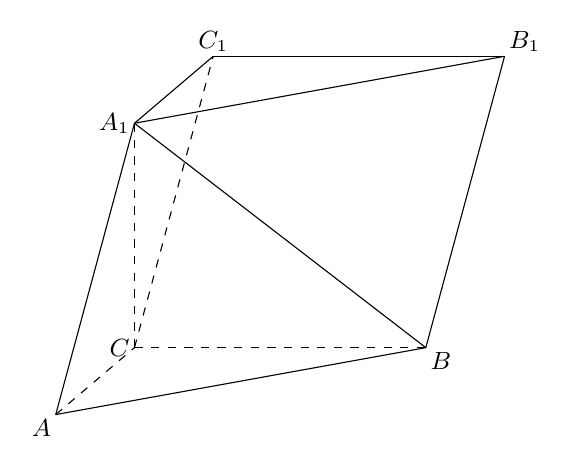
\begin{tikzpicture}[font=\small, line width=0.4pt,
  every node/.style={inner sep=1.5pt}]
  % 图纸坐标只用于复现原卷投影；上下两个三角形保持同一平移向量。
  \coordinate (A)  at (0,0);
  \coordinate (C)  at (1.00,0.85);
  \coordinate (B)  at (4.70,0.85);
  \coordinate (A1) at (1.00,3.70);
  \coordinate (C1) at (2.00,4.55);
  \coordinate (B1) at (5.70,4.55);

  % 遮挡棱及题设虚线先画，保证交叉处的可见实线在前。
  \draw[dashed] (A) -- (C);
  \draw[dashed] (C) -- (B);
  \draw[dashed] (C) -- (C1);
  \draw[dashed] (A1) -- (C);

  % 可见棱
  \draw (A) -- (B);
  \draw (A) -- (A1);
  \draw (A1) -- (C1);
  \draw (C1) -- (B1);
  \draw (B1) -- (B);
  \draw (A1) -- (B1);

  % 题面明确画出的线段 A1B
  \draw (A1) -- (B);

  % 顶点标注
  \node[anchor=north east] at (A)  {$A$};
  \node[anchor=east]       at (C)  {$C$};
  \node[anchor=north west] at (B)  {$B$};
  \node[anchor=east]       at (A1) {$A_1$};
  \node[anchor=south]      at (C1) {$C_1$};
  \node[anchor=south west] at (B1) {$B_1$};
\end{tikzpicture}
\end{center}
\nopagebreak[4]
  (1) 证明：平面 $ACC_1A_1\perp$ 平面 $BB_1C_1C$；

  (2) 设 $AB=A_1B$，$AA_1=2$，求四棱锥 $A_1-BB_1C_1C$ 的高．

\end{question}
\begin{question}
\gkti{19}一项试验旨在研究臭氧效应，试验方案如下：选 $40$ 只小白鼠，随机地将其中 $20$ 只分配到试验组，另外 $20$ 只分配到对照组，试验组的小白鼠饲养在高浓度臭氧环境，对照组的小白鼠饲养在正常环境，一段时间后统计每只小白鼠体重的增加量（单位：g）．试验结果如下：

对照组的小白鼠体重的增加量从小到大排序为

$15.2\quad18.8\quad20.2\quad21.3\quad22.5\quad23.2\quad25.8\quad26.5\quad27.5\quad30.1$

$32.6\quad34.3\quad34.8\quad35.6\quad35.6\quad35.8\quad36.2\quad37.3\quad40.5\quad43.2$

试验组的小白鼠体重的增加量从小到大排序为

$7.8\quad9.2\quad11.4\quad12.4\quad13.2\quad15.5\quad16.5\quad18.0\quad18.8\quad19.2$

$19.8\quad20.2\quad21.6\quad22.8\quad23.6\quad23.9\quad25.1\quad28.2\quad32.3\quad36.5$

  (1) 计算试验组的样本平均数；

  (2) ① 求 $40$ 只小白鼠体重的增加量的中位数 $m$，再分别统计两样本中小于 $m$ 与不小于 $m$ 的数据的个数，完成如下列联表：

\begin{center}
\begin{tabular}{ccc}
\toprule
 & $<m$ & $\geqslant m$ \\
\midrule
对照组 &  &  \\
试验组 &  &  \\
\bottomrule
\end{tabular}
\end{center}

　　② 根据①中的列联表，能否有 $95\%$ 的把握认为小白鼠在高浓度臭氧环境中与在正常环境中体重的增加量有差异？

\Needspace{10\baselineskip}
附：$K^2=\dfrac{n(ad-bc)^2}{(a+b)(c+d)(a+c)(b+d)}$，

\begin{center}
\begin{tabular}{cccc}
\toprule
$P(K^2\geqslant k)$ & $0.100$ & $0.050$ & $0.010$ \\
\midrule
$k$ & $2.706$ & $3.841$ & $6.635$ \\
\bottomrule
\end{tabular}
\end{center}

\end{question}
\begin{question}
\gkti{20}已知函数 $f(x)=ax-\dfrac{\sin x}{\cos^2x}$，$x\in\left(0,\dfrac\pi2\right)$．

  (1) 当 $a=1$ 时，讨论 $f(x)$ 的单调性；

  (2) 若 $f(x)+\sin x<0$，求 $a$ 的取值范围．

\end{question}
\begin{question}
\gkti{21}已知直线 $x-2y+1=0$ 与抛物线 $C:y^2=2px$（$p>0$）交于 $A$，$B$ 两点，$|AB|=4\sqrt{15}$．

  (1) 求 $p$；

  (2) 设 $F$ 为 $C$ 的焦点，$M$，$N$ 为 $C$ 上两点，且 $\overrightarrow{FM}\cdot\overrightarrow{FN}=0$，求 $\triangle MFN$ 面积的最小值．

\end{question}
\begin{question}
\gkti{22}已知点 $P(2,1)$，直线 $l:\begin{cases}x=2+t\cos\alpha,\\y=1+t\sin\alpha\end{cases}$（$t$ 为参数），$\alpha$ 为 $l$ 的倾斜角，$l$ 与 $x$ 轴正半轴、$y$ 轴正半轴分别交于点 $A$，$B$，且 $|PA|\cdot|PB|=4$．

  (1) 求 $\alpha$；

  (2) 以坐标原点为极点，$x$ 轴正半轴为极轴建立极坐标系，求 $l$ 的极坐标方程．

\end{question}
\begin{question}
\gkti{23}设 $a>0$，函数 $f(x)=2|x-a|-a$．

  (1) 求不等式 $f(x)<x$ 的解集；

  (2) 若曲线 $y=f(x)$ 与 $x$ 轴所围成的图形的面积为 $2$，求 $a$．

\end{question}